%%%%%%%%%%%%%%%%%%%%%%%%%%%%%%%%%%%%%%%%%
% Beamer Presentation
% LaTeX Template
% Version 1.0 (10/11/12)
%
% This template has been downloaded from:
% http://www.LaTeXTemplates.com
%
% License:
% CC BY-NC-SA 3.0 (http://creativecommons.org/licenses/by-nc-sa/3.0/)
%
%%%%%%%%%%%%%%%%%%%%%%%%%%%%%%%%%%%%%%%%%

%----------------------------------------------------------------------------------------
%	PACKAGES AND THEMES
%----------------------------------------------------------------------------------------

\documentclass[10pt]{beamer}

\mode<presentation> {

% The Beamer class comes with a number of default slide themes
% which change the colors and layouts of slides. Below this is a list
% of all the themes, uncomment each in turn to see what they look like.

\renewcommand{\familydefault}{\rmdefault}

\graphicspath{ {./figures/} }
\usepackage{graphicx} % Allows including images
\usepackage{booktabs} % Allows the use of \toprule, \midrule and \bottomrule in tables
\usepackage{tikz} % Allows the use of \toprule, \midrule and \bottomrule in tables
\usepackage{hyperref}
\usepackage{breqn}
\usepackage[printwatermark]{xwatermark}

\usetheme{default}
% \usetheme{AnnArbor}
% \usetheme{Antibes}
% \usetheme{Bergen}
% \usetheme{Berkeley}
% \usetheme{Berlin}
% \usetheme{Boadilla}
% \usetheme{CambridgeUS}
% \usetheme{Copenhagen}
% \usetheme{Darmstadt}
% \usetheme{Dresden}
% \usetheme{Frankfurt}
% \usetheme{Goettingen}
% \usetheme{Hannover}
% \usetheme{Ilmenau}
% \usetheme{JuanLesPins}
% \usetheme{Luebeck}
% \usetheme{Madrid}
% \usetheme{Malmoe}
% \usetheme{Marburg}
% \usetheme{Montpellier}
% \usetheme{PaloAlto}
% \usetheme{Pittsburgh}
% \usetheme{Rochester}
% \usetheme{Singapore}
% \usetheme{Szeged}
% \usetheme{Warsaw}

% As well as themes, the Beamer class has a number of color themes
% for any slide theme. Uncomment each of these in turn to see how it
% changes the colors of your current slide theme.

% \usecolortheme{albatross}
\usecolortheme{beaver}
% \usecolortheme{beetle}
% \usecolortheme{crane}
% \usecolortheme{dolphin}
% \usecolortheme{dove}
% \usecolortheme{fly}
% \usecolortheme{lily}
% \usecolortheme{orchid}
% \usecolortheme{rose}
% \usecolortheme{seagull}
% \usecolortheme{seahorse}
% \usecolortheme{whale}
% \usecolortheme{wolverine}

%\setbeamertemplate{footline} % To remove the footer line in all slides uncomment this line
\setbeamertemplate{footline}[page number] % To replace the footer line in all slides with a simple slide count uncomment this line

\setbeamertemplate{navigation symbols}{} % To remove the navigation symbols from the bottom of all slides uncomment this line

% \setbeamertemplate{background}{
%     \tikz[overlay,remember picture]\node[opacity=0.4]at (current page.center){
%         \includegraphics[width=2cm]{iot_analytics_logo.jpg}
%         }}

}

%----------------------------------------------------------------------------------------
%	TITLE PAGE
%----------------------------------------------------------------------------------------

\title[What Phone do People Like?]{Phone Sentiment Analysis with Web Crawl Data} % The short title appears at the bottom of every slide, the full title is only on the title page

\author{Tuomo Kareoja} % Your name
\institute[IOT Analytics] % Your institution as it will appear on the bottom of every slide, may be shorthand to save space
{
IOT Analytics \\ % Your institution for the title page
\medskip
}
\date{\today} % Date, can be changed to a custom date

\begin{document}

\begin{frame}
\titlepage % Print the title page as the first slide
\end{frame}

\begin{frame}
\frametitle{Agenda} % Table of contents slide, comment this block out to remove it
\tableofcontents % Throughout your presentation, if you choose to use \section{} and \subsection{} commands, these will automatically be printed on this slide as an overview of your presentation
\end{frame}

%----------------------------------------------------------------------------------------
%	PRESENTATION SLIDES
%----------------------------------------------------------------------------------------

%------------------------------------------------
\section{Background}
%------------------------------------------------

\begin{frame}
\frametitle{
    Background
}

\begin{itemize}
    \item Mission: Locate device by its WiFi fingerprint
    \item Area to cover:
    \begin{itemize}
        \item Three buildings of Universitat Jaume I with 4 or more floors and almost 110.000 m\(^2\)
        \item More than 20 different users and 25 Android devices, with widely varying signal strengths
        \item Area covered by 520 different WiFi access-points
    \end{itemize}
\end{itemize}


{
    \centering
    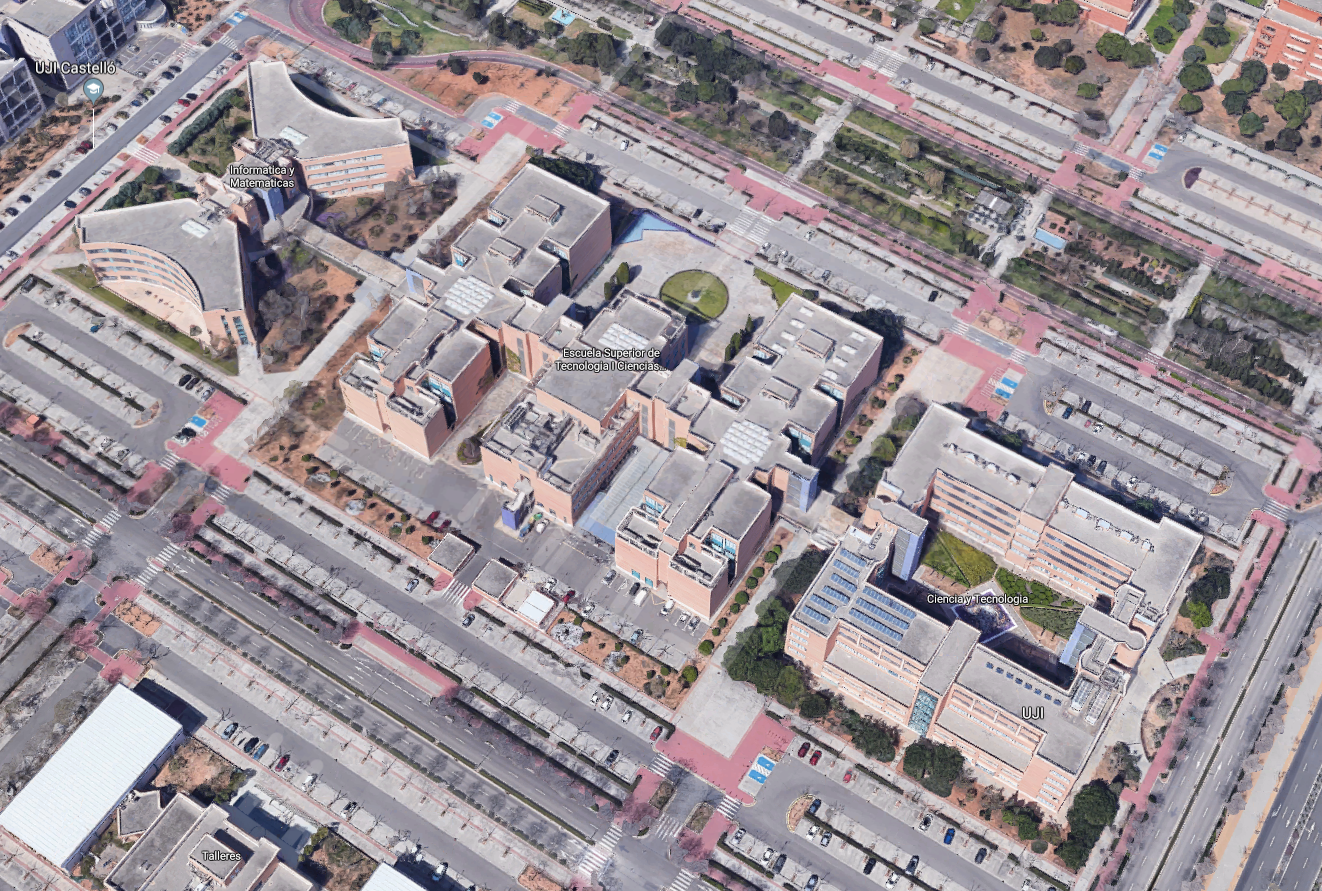
\includegraphics[width=8cm,keepaspectratio]{university_campus_gmaps.png}
    \par
}

\end{frame}

%------------------------------------------------
\section{Modelling}
%------------------------------------------------

\begin{frame}
\frametitle{Data Processing}

\begin{itemize}
    \item On top of WiFi signal strength also the phone model and OS very provided.
    These were not used in the models and dropped
    \item Missing signal for Wifi access-points was recoded from 100 to -110 so that
    it was smaller than the weakest actual signal in the dataset (-105)
    \item No scaling was done as all the models used where tree based
    \item outlier dropping was tried, but this led to worse performance, so all
    observations where kept in the analysis
\end{itemize}

\end{frame}

%------------------------------------------------
\subsection{Model Building}
%------------------------------------------------

\begin{frame}
\frametitle{Model Types Used}

\begin{itemize}
    \item Different variations of KNN models were tried as these usually perform well in
    in these locationing tasks and can predict multiple related targets
    (latitude, longitude, building, floor) all at once
    \begin{itemize}
        \item K and radius model uses 3 closest observations by similarity of
        WiFi signals, but beyond most nearest neighbor it only considers observations
        which are within certain radius limit of this distance
        \item KNN grouping model uses 2 closest observations by similarity of
        WiFi signals, but before training the models the WiFi signals strengths
        were grouped averaged for by room
    \end{itemize}
    \item Second option was to create multiple models to predict different metrics with
    interconnected CatBoost models that would capture the connections between
    target values
    \begin{enumerate}
        \item Separate model was created to predict each outcome from WiFi signals
        \item The predictions from previous models were added beside the Wifi signals
        and given to second layer of models that had the same goal as the first ones
        \item Lastly the just predictions from the second layer were given to
        a last layer of 4 models that made the final prediction
    \end{enumerate}
\end{itemize}

\end{frame}

\begin{frame}
\frametitle{Model Evaluation}

Models were evaluated by a single scoring metrics named Distance 75 that combines all
the 4 target values. This metric calculates the manhattan distance between prediction
and actual values in 3D spaces and adds a additional penalty for getting the
building wrong:

\bigskip

Distance75 =

\begin{dmath}
\frac{1}{n}*\sum_{n=1}^{n}(|longitude_{predicted}-longitude_{actual}|\\
+|latitude_{predicted}-latitude_{actual}| \\
+4*|floor\:number_{predicted}-floor\:number_{actual}| \\
+50*|building\:number_{predicted}-building\:number_{actual}|)
\end{dmath}

\end{frame}

%------------------------------------------------
\subsection{Model Performance}
%------------------------------------------------

\begin{frame}
\frametitle{Overall Performance}

\begin{itemize}
    \item KNN models perform clearly much better than CatBoost
    \item Building is easy to predict, but floor is not
\end{itemize}

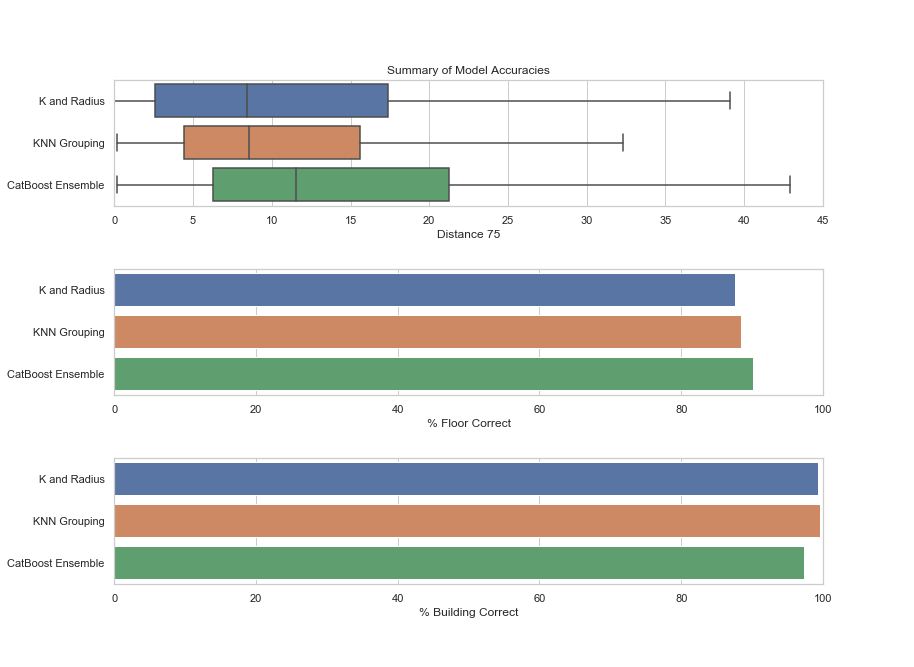
\includegraphics[width=\textwidth,height=\textheight,keepaspectratio]{error_summary.png}

\end{frame}

\begin{frame}
\frametitle{Error distribution}

\begin{itemize}
    \item K and radius model has a fatter tail than KNN grouping in errors
\end{itemize}

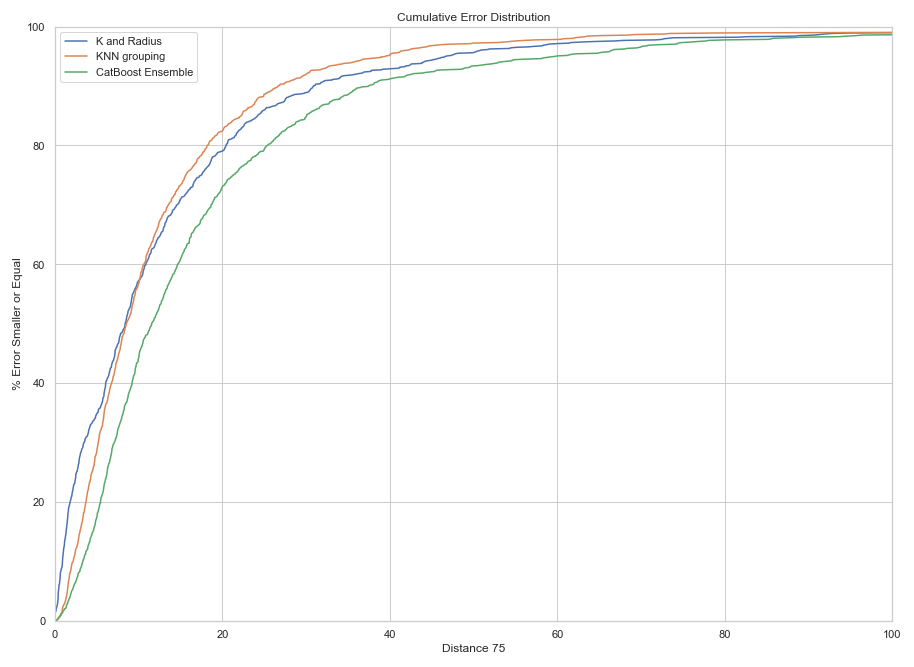
\includegraphics[width=\textwidth,height=\textheight,keepaspectratio]{error_cumulative.png}

\end{frame}


\begin{frame}
\frametitle{KNN models vs. CatBoost}

\begin{itemize}
    \item CatBoost makes predictions that are outside the buildings
\end{itemize}

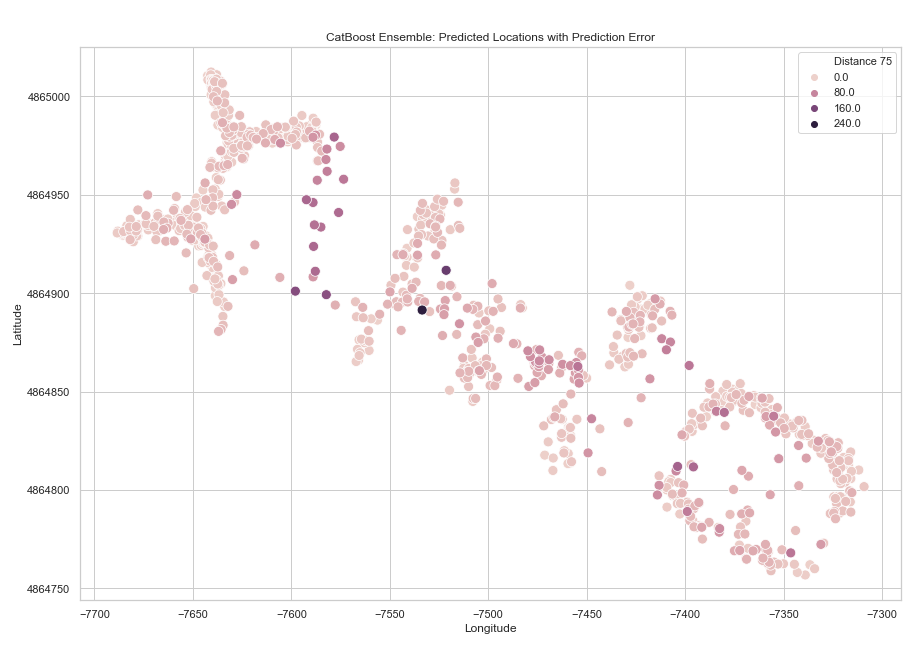
\includegraphics[width=\textwidth,height=\textheight,keepaspectratio]{catboost_ensemble_error_of_predicted_locations.png}

\end{frame}

\begin{frame}
\frametitle{KNN models vs. CatBoost}

\begin{itemize}
    \item KNN keeps to already observed values and makes no stupid errors
\end{itemize}

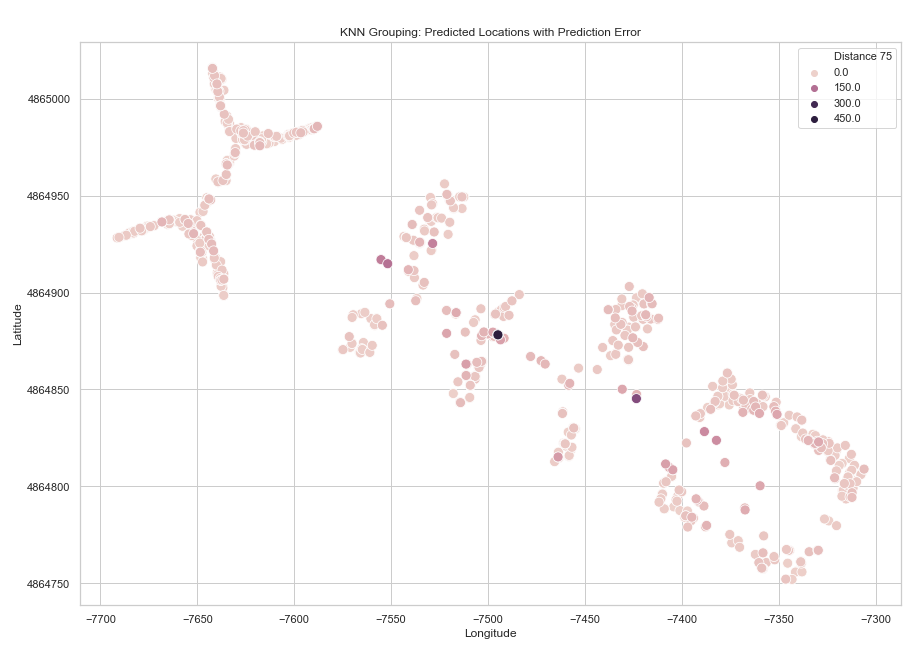
\includegraphics[width=\textwidth,height=\textheight,keepaspectratio]{knn_grouping_error_of_predicted_locations.png}

\end{frame}

%------------------------------------------------
\section{Conclusion}
%------------------------------------------------

\begin{frame}
\frametitle{Conclusions}

\begin{enumerate}
    \item If we have have identifiers for unique locations (e.g. rooms and hallways) in the final
    training data, then KNN model with grouping is the best choice. It is also smaller than normal KNN
    model be an order or magnitude and so much faster with its predictions
    \item If the final training data does not identifiers for unique locations or we get more
    training data in the future that does not have these labels, then K and radius model is the best
    choice
    \item Hard to model as the model has to be able to predict multiple related targets (
        e.g. longitude and latitude)
    \item Simple KNN model with some adjustment beats more complex models
    \item Signal processing does not seem to help (maybe should be done for each OS separately)
\end{enumerate}

\end{frame}

\begin{frame}
\frametitle{The End}

\LARGE{\centerline{Questions?}}

\end{frame}

%----------------------------------------------------------------------------------------

\end{document}
